% --------------------------------------------------------------
% This is all preamble stuff that you don't have to worry about.
% Head down to where it says "Start here"
% --------------------------------------------------------------
 
\documentclass[12pt]{article}
 
\usepackage[margin=1in]{geometry} 
\usepackage{bm} % bold in mathmode \bm
\usepackage{amsmath,amsthm,amssymb,mathtools}
\usepackage{dsfont} % for indicator function \mathds 1
\usepackage{mathdots} % for \iddots
\usepackage{tikz,pgf,pgfplots}
\usepackage{enumerate} 
\usepackage[multiple]{footmisc} % for an adjascent footnote
\usepackage{graphicx,float} % figures
\usepackage{framed} % surround a text with a box 
\usepackage{changepage} % \begin{adjustwidth}{2cm}{} environment

\newtheorem{definition}{Definition}
\let\olddefinition\definition
\renewcommand{\definition}{\olddefinition\normalfont}
\newtheorem{lemma}{Lemma}
\let\oldlemma\lemma
\renewcommand{\lemma}{\oldlemma\normalfont}
\newtheorem{proposition}{Proposition}
\let\oldproposition\proposition
\renewcommand{\proposition}{\oldproposition\normalfont}
\newtheorem{corollary}{Corollary}
\let\oldcorollary\corollary
\renewcommand{\corollary}{\oldcorollary\normalfont}
\newtheorem{theorem}{Theorem}
\let\oldtheorem\theorem
\renewcommand{\theorem}{\oldtheorem\normalfont}

%%% PLOTTING PARAMETERS
\tikzstyle{bag} = [text width=7em, text centered] %% binomial tree node width
\tikzstyle{end} = []

\pgfplotsset{soldot/.style={color=black,only marks,mark=*},
             holdot/.style={color=black,fill=white,only marks,mark=*},
             compat=1.12}
%%%

%% I want to be in control of when to indent...
%% set noindent as the default status and define \indent to indent a line
\newlength\tindent
\setlength{\tindent}{\parindent}
\setlength{\parindent}{0pt}
\renewcommand{\indent}{\hspace*{\tindent}}

\newcommand*{\vv}[1]{\vec{\mkern0mu#1}} % \vec command

%% DAVIDS MACRO KIT %%
\newcommand{\R}{\mathbb R}
\newcommand{\N}{\mathbb N}
\newcommand{\Z}{\mathbb Z}
\renewcommand{\P}{\mathbb P}
\newcommand{\Q}{\mathbb Q}
\newcommand{\E}{\mathbb E}
\newcommand{\var}{\mathrm{Var}}
\newcommand{\Var}{\mathrm{Var}}
\newcommand{\cov}{\mathrm{Cov}}
\newcommand{\Cov}{\mathrm{Cov}}
\newcommand{\indist}{\,{\buildrel \mathcal D \over \sim}\,}

\newcommand{\bigtau}{\text{{\large $\bm \tau$}}}

\begin{document}
 
% --------------------------------------------------------------
%                         Start here
% --------------------------------------------------------------
 
\title{Mathematical \& Computational Finance I\\Lecture Notes}
\author{Interest-Rate-Dependent Assets}
\date{March 22 2016 \\ Last update: \today{}}
\maketitle

% SECTION: 
\section{Introduction}

\indent Up to now we have been assuming constant values for our riskless rate with which we discount by. In this section we ask what if we relax this assumption and permit stochastic rates? In the real-world constant rates may be used: If we consider sufficiently short time frames then we often allow our models to use constant rates. However, for any sufficiently long time frame it is significantly more realistic to let out rates fluctuate through time. The interest rate model we use will be an {\em idealized} version of the true interest rate. As is with any model, we are required to make some modelling assumptions. In particular, we will consider a binomial model for interest rates similar to that used in our asset model. \\

\indent Interest rate models are particularly important when used in combination with models for other underlying asset classes \& long-term financial obligations (i.e. pensions, insurance, etc.). \\

\indent For the remainder of these notes let $\Omega$ be the set of $2^N$ possible outcomes $\omega_1\cdots\omega_N$ of $N$ tosses of a coin. Define $\tilde{\P}$ to be a probability measure of $\Omega$. At this moment $\tilde{\P}$ may be any probability measure, but ultimately $\tilde{\P}$ will be our risk-neutral measure.  \\

\begin{definition} An \underline{interest rate process} is a sequence of random variables
\begin{equation*}
	R_0,\,R_1,\, \cdots,\, R_{N - 1}
\end{equation*}

where $R_0$ is a non-random constant. For $n = 1,...,N - 1$ the random variable $R_n$ depends only on the first $n$ coin tosses $\omega_1\cdots\omega_n$. That is, the interest rate at time $n$ depends only on the interest rates preceding it.
\end{definition} \hfill\\

\indent A direct consequence of this definition we have that one dollar invested in a bank account at time $n$ for rate $R_n$ will grow to $(1 + R_n)$ at time $n + 1$. Note that if we invest in the bank account at time $n$ will we know in advance the value that the investment will take at time $n + 1$. \\

\begin{definition} Similar to our asset process studied earlier we find the interest rate process to be an adapted process. However, while the interest rate process is adapted we say that the portfolio value of an investment under the interest rate process is a \underline{predictable process}. That is, we will know the value the process will be a step before it reaches the value. \\

\indent More precisely, a \underline{predictable process} is any stochastic process whose value depends on the information up to an earlier time. So, if $X_n$ is a predictable process then we have that
\begin{equation*}
	X_n = X_n(\omega_1\cdots\omega_{n - k}) \quad \text{for } 1 \leq k \leq n
\end{equation*}
\end{definition} \hfill\\

Typically, we require that $R_n(\omega_1\cdots\omega_n) > 0$. However, for now we only require
\begin{equation*}
	R_n(\omega_1\cdots\omega_n) > 0 \quad \forall\,n = 0,1,...,N,~\omega_1\cdots\omega_n \in \Omega
\end{equation*}
unless otherwise specified. \\

\begin{definition} Define the \underline{discount process}
\begin{equation*}
	D_n = \frac{1}{ (1 + R_0)(1 + R_1) \cdots (1 + R_{n - 1})} = \frac{1}{ \prod^n_{j = 0} (1 + R_j) }
\end{equation*}

for $n = 1,2,...,N$ and with $D_0 = 1$. We observe that since $D_n$ depends on only the first $(n - 1)$ coin tosses $\omega_1\cdots\omega_{n - 1}$ then we have that $D_n$ is a predictable process.
\end{definition} \hfill\\

\indent If $\tilde{\P}$ is the risk-neutral measure then the risk-neutral pricing formula should give us that the time-zero value of a payment $X$ received at time $m$ will be
\begin{equation*}
	\tilde{\E}_0 \left[ \frac{X}{ \prod^m_{j = 0} (1 + R_j) } \right] = \tilde{\E}[D_m X]
\end{equation*}

where $X$ may only depend on $\omega_1\cdots\omega_m$. \\

\subsection{Model Choice}

\indent Our approach will begin with constructing a zero-coupon bond, reflecting the existence of zero-coupon bonds at specific maturities found in the market. However, we cannot {\em ipso facto} preclude arbitrage between these zero-coupon instruments of different maturities. With this in mind we should note that in order to build pricing and hedging models we require a model free of arbitrage. That is, if we permit arbitrage then what should the rational price of a derivative be where we may begin with zero initial wealth and hedge a short position via market arbitrage? In principle, we could argue that the rational price under such assumptions should be zero, which clearly doesn't suit our purposes. \\

\indent In this section we address the issue of arbitrage by constructing our model under the risk-neutral measure. That is, we describe a process for which describe our interest rate in the risk-neutral world and then price derivatives dependent on this rate under the same measure using risk-neutral pricing. By doing so we are guaranteed that all discounted asset prices must be martingales, and thereby guaranteed that discounted portfolio processes must be martingales.\footnote{Proven later in the section.}~By definition a martingale beginning at zero must have expectation zero. By this we find that martingales are inconsistent with arbitrage since they cannot take positive value with positive probability without also taking negative value with positive probability. \\

\indent Once we price our instrument under the risk-neutral measure we, in principle, demonstrate that we can perform a change of measure to the real-world measure to give us real-world results. \\

\indent Alternatively, we could start from interest rates and use the risk-neutral pricing directly are called \underline{short-rate models}. An example of such a model would be to first describe the evolution of a random yield curve and then construct the conditions under which this model would satisfy no-arbitrage.

\section{Binomial Model for Interest Rates}

\begin{definition} The time-zero price of a \underline{zero-coupon bond} that pays $\$1$ at maturity $m$ is given by
\begin{equation*}
	B_{0,m} = \tilde{\E}[D_m]
\end{equation*}

The \underline{yield} for a zero-coupon bond maturing at time $m$ is the value $y_m$ such that
\begin{equation*}
	\frac{1}{B_{0,m}} = (1 + y_m)^m
\end{equation*}

which can be thought of the number of units of the bond that can be purchased for $\$1$. That is, an investment of $\$1$ in the $m$ maturity bond would purchase $\frac{1}{B_{0,m}}$ bonds with payoff $\frac{1}{B_{0,m}}$ at time $m$. \\

\indent The yield $y_m$ is the equivalent constant period interest rate between time 0 and time $m$ such that $\$1$ invested at time zero for $m$ periods will grow to $\frac{1}{B_{0,m}}$ at time $m$.
\end{definition} \hfill\\

With this definition for $y_m$ we have that
\begin{equation*}
	y_m = \left( \frac{1}{B_{0,m}} \right)^\frac{1}{m} - 1
\end{equation*}

\underline{Example:} Suppose $N = 3$ and we are given that
\begin{align*}
	\tilde{\P}(HHH) &= \frac{2}{9} \\
	\tilde{\P}(HHT) &= \frac{1}{9},~\tilde{\P}(HTH) = \frac{1}{12},~\tilde{\P}(THH) = \frac{1}{6} \\
	\tilde{\P}(HTT) &= \frac{1}{12},~\tilde{\P}(THT) = \frac{1}{12},~\tilde{\P}(TTH) = \frac{1}{8} \\			
	\tilde{\P}(TTT) &= \frac{1}{8}	
\end{align*}

Define the sets
\begin{align*}
	A_{HH} &= \left\{\omega_1 = H, \omega_2 = H \right\} = \left\{HHH, HHT \right\} \\
	A_{HT} &= \left\{\omega_1 = H, \omega_2 = T \right\} = \left\{HTH, HTT \right\} \\
	A_{TH} &= \left\{\omega_1 = T, \omega_2 = H \right\} = \left\{THH, THT \right\} \\
	A_{TT} &= \left\{\omega_1 = T, \omega_2 = T \right\} = \left\{TTH, TTT \right\}	
\end{align*}

Then
\begin{align*}
	\tilde{\P}(A_{HH}) &= \tilde{\P}\left( HHH, HHT \right) \\
	&= \tilde{\P}\left(HHH \cup HHT \right) \\
	&= \tilde{\P}(HHH) + \tilde{\P}(HHT) \\
	&= \frac{2}{9} + \frac{1}{9} \\
	&= \frac{1}{3} \\
	\tilde{\P}(A_{HT}) &= \frac{1}{6} \\
	\tilde{\P}(A_{TH}) &= \frac{1}{4} \\
	\tilde{\P}(A_{TT}) &= \frac{1}{4}
\end{align*}

Also define
\begin{align*}
	A_H &= \left\{\omega_1 = H \right\} = \left\{HHH, HHT, HTH, HTT \right\} \\
	A_T &= \left\{\omega_2 = T \right\} = \left\{THH, THT, TTH, TTT \right\}
\end{align*}

Then
\begin{align*}
	\tilde{\P}(A_H) &= \tilde{\P}(HHH, HHT, HTH, HTT) \\
	&= \tilde{\P}( HHH, HHT, HTH, HTT ) \\
	&= \tilde{\P}( HHH \cup HHT \cup HTH \cup HTT ) \\
	&= \tilde{\P}(HHH) + \tilde{\P}(HHT) + \tilde{\P}(HTH) + \tilde{\P}(HTT) \\
	&= \frac{2}{9} + \frac{1}{9} + \frac{1}{12} + \frac{1}{12} \\
	&= \frac{1}{2} \\
	\tilde{\P}(A_T) &= \frac{1}{2}
\end{align*}

Recall that 
\begin{equation*}
	\P(A~|~B) = \frac{ \P(A\cap B) }{ \P(B) }
\end{equation*}

Then, conditional on the first coin toss $\omega_1$ we find the two step transitions
\begin{align*}
	\tilde{\P}(\omega_3 = H~|~\omega_1 = H,\omega_2 = H) &= \frac{ \tilde{\P}(HHH) }{ \tilde{\P}(A_{HH}) } = \frac{ \frac{2}{9} }{ \frac{1}{3} } = \frac{2}{3}	 \\
	\tilde{\P}(\omega_3 = T~|~\omega_1 = H,\omega_2 = H) &= \frac{ \tilde{\P}(HHT) }{ \tilde{\P}(A_{HH}) } = \frac{ \frac{1}{9} }{ \frac{1}{3} } = \frac{1}{3} \\
	\tilde{\P}(\omega_3 = H~|~\omega_1 = H,\omega_2 = T) &= \frac{ \tilde{\P}(HTH) }{ \tilde{\P}(A_{HT}) } = \frac{ \frac{1}{12} }{ \frac{1}{6} } = \frac{1}{2} \\
	\tilde{\P}(\omega_3 = T~|~\omega_1 = H,\omega_2 = T) &= \frac{ \tilde{\P}(HTT) }{ \tilde{\P}(A_{HT}) } = \frac{ \frac{1}{12} }{ \frac{1}{6} } = \frac{1}{2} \\
	\tilde{\P}(\omega_3 = H~|~\omega_1 = T,\omega_2 = H) &= \frac{ \tilde{\P}(THH) }{ \tilde{\P}(A_{TH}) } = \frac{ \frac{1}{6} }{ \frac{1}{4} } = \frac{2}{3} \\
	\tilde{\P}(\omega_3 = T~|~\omega_1 = T,\omega_2 = H) &= \frac{ \tilde{\P}(THT) }{ \tilde{\P}(A_{TH}) } = \frac{ \frac{1}{12} }{ \frac{1}{4} } = \frac{1}{3}	 \\
	\tilde{\P}(\omega_3 = H~|~\omega_1 = T,\omega_2 = T) &= \frac{ \tilde{\P}(TTH) }{ \tilde{\P}(A_{TT}) } = \frac{ \frac{1}{8} }{ \frac{1}{4} } = \frac{1}{2}	\\
	\tilde{\P}(\omega_3 = T~|~\omega_1 = T,\omega_2 = T) &= \frac{ \tilde{\P}(TTT) }{ \tilde{\P}(A_{TT}) } = \frac{ \frac{1}{8} }{ \frac{1}{4} } = \frac{1}{2}
\end{align*}

and conditional on the first coin toss $\omega_1$ we find the one step transitions
\begin{align*}
	\tilde{\P}(\omega_2 = H~|~\omega_1 = H) &= \frac{ \tilde{\P}(A_{HH}) }{ \tilde{\P}(A_{H}) } = \frac{ \frac{1}{3} }{ \frac{1}{2} } = \frac{2}{3} \\
	\tilde{\P}(\omega_2 = T~|~\omega_1 = H) &= \frac{ \tilde{\P}(A_{HT}) }{ \tilde{\P}(A_{H}) } = \frac{ \frac{1}{6} }{ \frac{1}{2} } = \frac{1}{3} \\
	\tilde{\P}(\omega_2 = H~|~\omega_1 = T) &= \frac{ \tilde{\P}(A_{TH}) }{ \tilde{\P}(A_{T}) } = \frac{ \frac{1}{4} }{ \frac{1}{2} } = \frac{1}{2} \\
	\tilde{\P}(\omega_2 = T~|~\omega_1 = T) &= \frac{ \tilde{\P}(A_{TT}) }{ \tilde{\P}(A_{T}) } = \frac{ \frac{1}{4} }{ \frac{1}{2} } = \frac{1}{2}		
\end{align*}

From these probabilities we may compute the following interest rate process
\begin{figure}[H]
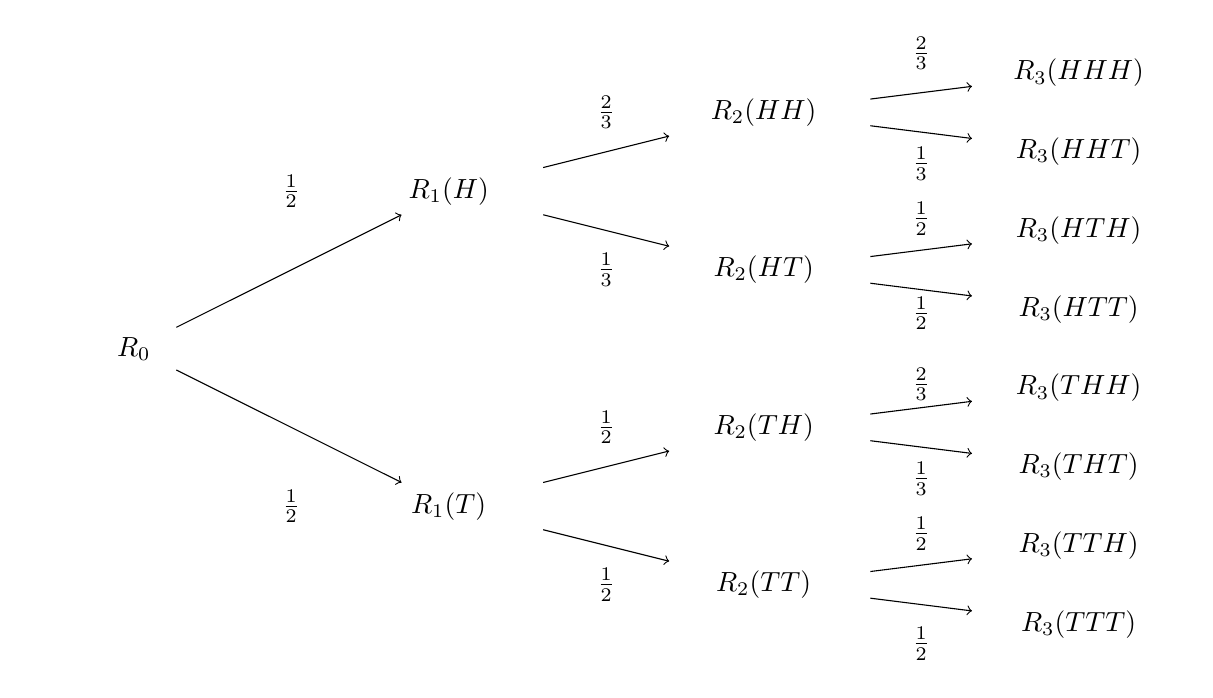
\begin{tikzpicture}[sloped]
  \node (a) at (0,0) [bag] {$R_0$};
  \node (b) at (4,-2) [bag] {$R_1(T)$};
  \node (c) at (4,2) [bag] {$R_1(H)$};
  \node (d) at (8,-3) [bag] {$R_2(TT)$};
  \node (e) at (8,-1) [bag] {$R_2(TH)$};
  \node (f) at (8,1) [bag] {$R_2(HT)$};
  \node (g) at (8,3) [bag] {$R_2(HH)$};
  \node (h) at (12,-3.5) [bag] {$R_3(TTT)$};
  \node (i) at (12,-2.5) [bag] {$R_3(TTH)$};
  \node (j) at (12,-1.5) [bag] {$R_3(THT)$};
  \node (k) at (12,-0.5) [bag] {$R_3(THH)$};
  \node (l) at (12,0.5) [bag] {$R_3(HTT)$};
  \node (m) at (12,1.5) [bag] {$R_3(HTH)$};
  \node (n) at (12,2.5) [bag] {$R_3(HHT)$};
  \node (o) at (12,3.5) [bag] {$R_3(HHH)$};
  
  \node at (2,-2) {$\frac{1}{2}$};
  \draw [->] (a) to node [below] {} (b);
  \node at (2,2) {$\frac{1}{2}$};  
  \draw [->] (a) to node [above] {} (c);
  \node at (6,-3) {$\frac{1}{2}$};
  \draw [->] (b) to node [below] {} (d);
  \node at (6,-1) {$\frac{1}{2}$};
  \draw [->] (b) to node [above] {} (e);
  \node at (6,1) {$\frac{1}{3}$};
  \draw [->] (c) to node [below] {} (f);
  \node at (6,3) {$\frac{2}{3}$};  
  \draw [->] (c) to node [above] {} (g);
  \node at (10,-3.75) {$\frac{1}{2}$};
  \draw [->] (d) to node [below] {} (h);
  \node at (10,-2.35) {$\frac{1}{2}$};
  \draw [->] (d) to node [above] {} (i);
  \node at (10,-1.65) {$\frac{1}{3}$};
  \draw [->] (e) to node [below] {} (j);
  \node at (10,-0.45) {$\frac{2}{3}$};  
  \draw [->] (e) to node [above] {} (k);
  \node at (10,0.45) {$\frac{1}{2}$};  
  \draw [->] (f) to node [below] {} (l);
  \node at (10,1.65) {$\frac{1}{2}$};
  \draw [->] (f) to node [above] {} (m);
  \node at (10,2.35) {$\frac{1}{3}$};
  \draw [->] (g) to node [above] {} (n);
  \node at (10,3.75) {$\frac{2}{3}$};    
  \draw [->] (g) to node [above] {} (o);  
\end{tikzpicture}
\caption{Interest rate process with conditional transition probabilities annotated above each branch.}
\end{figure}

\indent We call such conditional probabilities the {\em transition probabilities} associated with $\tilde{\P}$. Recall that, from basic probability, we have
\begin{align*}
	\P(A\cap B ~|~ C) &= \frac{ \P(A\cap B\cap C) }{ \P(C) } \\
	&= \frac{ \P(A ~|~ B \cap C) \cdot \P(B\cap C) }{ \P(C) }	 \\
	&= \P( A~|~B\cap C) \cdot \P(B~|~C)
\end{align*}

From this we can also compute conditional probabilities of joint events such as
\begin{equation*}
	\tilde{\P}(\omega_2 = H, \omega_3 = H~|~\omega_1 = H)
\end{equation*}

by multiplying
\begin{equation*}
	\tilde{\P}(\omega_2 = H~|~\omega_1 = H)\cdot \tilde{\P}(\omega_3 = H~|~\omega_1 = H, \omega_2 = H) = \frac{2}{3}\cdot\frac{2}{3} = \frac{4}{9}
\end{equation*}

Alternatively we could have used
\begin{align*}
	\P(A\cap B ~|~ C) &= \frac{ \P(A\cap B\cap C) }{ \P(C) } \\
	\implies \tilde{\P}(\omega_2 = H, \omega_3 = H~|~\omega_1 = H) &= \frac{ \tilde{\P}(HHH) }{ \tilde{\P}(A_H) } = \frac{ \frac{2}{9} }{ \frac{1}{2} } = \frac{4}{9}
\end{align*}

Now, let $X$ be a random variable depending on three coin tosses $\omega_1\omega_2\omega_3$. From these probabilities we can compute various conditional expectations, for example,
\begin{align*}
	\tilde{\E}_1[X](H) &= X(HHH)\tilde{\P}(\omega_2 = H,\omega_3 = H~|~\omega_1 = H)~+ \\
	&\hphantom{{}={---}} X(HHT)\tilde{\P}(\omega_2 = H, \omega_3 = T~|~\omega_1 = H)~+ \\
	&\hphantom{{}={---}} X(HTH)\tilde{\P}(\omega_2 = T, \omega_3 = H~|~\omega_1 = H)~+ \\
	&\hphantom{{}={---}} X(HTT)\tilde{\P}(\omega_2 = T, \omega_3 = T~|~\omega_1 = H)
\end{align*} \\

\indent We wish to generalize the notion of conditional expectation to the case of non-independent coin tosses. For this purpose we introduce the following definition:

\begin{definition} Let $\tilde{\P}$ be a probability measure on the space $\Omega$ of all sequences of $N$ coin tosses. Assume that $\tilde{\P}(\omega_1\cdots\omega_N) > 0$ for all $\omega_1\cdots\omega_N \in \Omega$.

Let $1 \leq n \leq N - 1$ and fix a coin toss sequence $\bar{\omega}_1 \cdots \bar{\omega}_N$. Then, we may define
\begin{equation*}
	\tilde{\P}( \omega_{n + 1} = \bar{\omega}_{n + 1},\cdots \omega_N = \bar{\omega}_N ~|~ \omega_1 = \bar{\omega}_1,\cdots,\omega_n = \bar{\omega}_n) = \frac{ \tilde{\P}(\bar{\omega}_1 \cdots \bar{\omega}_n\bar{\omega}_{n + 1} \cdots \bar{\omega}_N) }{ \tilde{\P}(\omega_1 = \bar{\omega}_1, \cdots, \omega_n = \bar{\omega}_n) }
\end{equation*}

Let $X$ be a random variable depending on $\omega_1\cdots\omega_N$. The conditional expectation of $X$ based on the information at time $n$ is defined as
\begin{align*}
	&\tilde{\E}_n[X](\bar{\omega}_1\cdots\bar{\omega}_n) = \\
	&\hphantom{{}={}} \sum_{\bar{\omega}_{n + 1}\cdots\bar{\omega}_N} X(\bar{\omega}_1\cdots\bar{\omega}_n\bar{\omega}_{n + 1}\cdots \bar{\omega}_N) \cdot \tilde{\P}(\omega_{n + 1} = \bar{\omega}_{n + 1}, \cdots, \omega_N = \bar{\omega}_N ~|~ \omega_1 = \bar{\omega}_1, \cdots, \omega_n = \bar{\omega}_n)
\end{align*}
\end{definition}

and, in particular, we have
\begin{align*}
	\tilde{\E}_0[X] &= \tilde{\E}[X] \\
	\tilde{\E}_N[X] &= X
\end{align*} \\

\begin{definition} Let $\tilde{\P}$ be a probability measure on $\Omega$ and let $R_0,R_1,...,R_{N - 1}$ be an interest rate process with each $R_n$ depending only on the first $n$ coin tosses satisfying $R_n > -1$. Recall that we had defined the discount process $D_n$ by
\begin{equation*}
	D_n = \frac{1}{\prod^{n - 1}_{i = 0} (1 + R_i) }, \quad n = 1,2,...,N;~ \text{with } D_0 = 1
\end{equation*}

\indent Then, for $0 \leq n \leq m \leq N$ the price at time $n$ of a \underline{zero-coupon bond} maturing at time $m$ is given by
\begin{equation*}
	B_{n,m} = \tilde{\E}_n \left[ \frac{D_m}{D_n} \right]
\end{equation*}
\end{definition}

Note that under this definition we have that
\begin{align*}
	B_{m,m} &= \tilde{\E}_m \left[ \frac{D_m}{D_m} \right] \\
	&= \tilde{\E}_m \left[ 1 \right] \\
	&= 1
\end{align*}

\indent Since $D_n$ is a function of $\omega_1\cdots\omega_{n - 1}$ we may `take out what is known' and express the bond price as
\begin{equation*}
	D_nB_{n,m} = \tilde{\E}_n[D_m]
\end{equation*}

\begin{proposition} The discounted bond price process $\left\{ D_nB_{n,m} \right\}^m_{n = 0}$ is a martingale under $\tilde{\P}$. 

\begin{proof} We first note that $D_nB_{n,m}$ must be adapted\footnote{Adapted to the first $n$ coin tosses? Or is it the first $n$ coin tosses?} since $D_nB_{n,m} = \tilde{\E}_n[D_m]$ and $D_m$ is a function of the first $m - 1$ coin tosses. Then, to check the martingale property we note that for $0 \leq k \leq n \leq m$ we have
\begin{align*}
	\tilde{\E}_k[D_nB_{n,m}] &= \tilde{\E}_k \left[ D_n \tilde{\E}_n \left[ \frac{D_m}{D_n} \right] \right] \quad \text{(by definition)} \\
	&= \tilde{\E}_k \left[ \tilde{\E}_n [D_m] \right] \quad \text{(taking out what is known)} \\
	&= \tilde{\E}_k [D_m] \quad \text{(tower property)} \\
	&= D_kB_{k,m} \quad \text{(by definition)}
\end{align*}

as desired.
\end{proof}
\end{proposition}

\indent Consider an individual who is able to trade in a zero-coupon bond of any maturity and the bank account. We can show that the discounted wealth of such an agent is a $\tilde{\P}$-martingale. Hence, there may not be arbitrage in the model with zero-coupon bonds as above. In general, we have that investing in the riskless bank account is no different from investing in the bond maturing in one period. \\

\indent Now, let $\Delta_{n,m}$, with $n < m$, be the number of $m$-maturity zero-coupon bonds held by an agent between times $n$ and $n + 1$. We only allow $\Delta_{n,m}$ to depend on the first $n$ coin tosses. \\

\indent Beginning with initial wealth $X_0$ at time $n = 0$ we say that the agent's wealth evolves according to the following wealth process/equation
\begin{equation*}
	X_{n + 1} = 1\cdot\Delta_{n,n + 1} + \sum^N_{m = n + 2} \Delta_{n,m}B_{n + 1,m} + (1 + R_n)\left[X_n - \sum^N_{m = n + 1} \Delta_{n,m}B_{n,m} \right]
\end{equation*}

where the initial 1 represents the face value of the bond.

\begin{theorem} Regardless of how the parameters of the portfolio variables are chosen, but subject to the constraint that $\Delta_{n,m}$ may depend only on the first $n$ coin tosses, the discounted wealth process $\left\{D_nX_n\right\}^N_{n = 0}$ is a $\tilde{\P}$-martingale where $X_n$ is given by the wealth equation immediately above.

\begin{proof} \underline{Adaptedness:} Note that our quantity $X_nD_n$ is adapted since $D_n$ depends only on the first $n - 1$ coin tosses $\omega_1\cdots\omega_{n - 1}$ and $X_n$ depends only on the first $n$ coin tosses since each component
\begin{equation*}
	X_n = 1\cdot\Delta_{n - 1,n} + \sum^N_{m = n + 1} \Delta_{n - 1,m}B_{n,m} + (1 + R_{n - 1})\left[X_{n - 1} - \sum^N_{m = n} \Delta_{n - 1,m}B_{n - 1,m} \right]
\end{equation*}

depends on the outcome of either the first $n - 1$ coin tosses or the first $n$ coin tosses. Rigorously we should be proving this inductively on $n$, with the base case being that $X_0$ is trivially adapted since it depends on no coin toss outcomes. \\

\underline{Martingale property:} Fix $n$ and consider the conditional expectation
\begin{align*}
	\tilde{\E}_n \left[ X_{n + 1} \right] &= \tilde{\E}_n \left[ 1\cdot\Delta_{n,n + 1} + \sum^N_{m = n + 2} \Delta_{n,m}B_{n + 1,m} + (1 + R_n)\left[X_n - \sum^N_{m = n + 1} \Delta_{n,m}B_{n,m} \right] \right] \\
	&= \tilde{\E}_n \left[ 1\cdot\Delta_{n,n + 1} \right] + \sum^N_{m = n + 2} \tilde{\E}_n \left[ \Delta_{n,m}B_{n + 1,m} \right] + \tilde{\E}_n \left[ (1 + R_n) \left[X_n - \sum^N_{m = n + 1} \Delta_{n,m}B_{n,m} \right] \right] \\
	&\hphantom{{}={--------------------------}} \quad \text{(linearity)}
\end{align*}

\indent Now note that $\Delta_{n,n + 1}$ in the first expectation is adapted to the first $n$ coin tosses, $\Delta_{n,m}B_{n + 1,m}$ in the second expectation is adapted to the first $n$ coin tosses, and $(1 + R_n)$, $X_n$, $\Delta_{n,m}B_{n,m}$ in the final expectation is adapted to the first $n$ coin tosses. So, we perform `taking out what is known' to get
\begin{align*}
	\tilde{\E}_n[X_{n + 1}] 	&= \Delta_{n, n + 1} + \sum^N_{m = n + 2} \Delta_{n,m} \tilde{\E}_n \left[ B_{n + 1,m}  \right] + (1 + R_n) \left( X_n - \sum^N_{m = n + 1} \Delta_{n,m}B_{n,m} \right) \\
	&= \Delta_{n, n + 1} + \sum^N_{m = n + 2} \Delta_{n,m} \tilde{\E}_n \left[ \frac{D_{n + 1}}{D_{n + 1}} B_{n + 1,m}  \right] + (1 + R_n) \left( X_n - \sum^N_{m = n + 1} \Delta_{n,m}B_{n,m} \right) \\
	&= \Delta_{n, n + 1} + \sum^N_{m = n + 2} \Delta_{n,m} \frac{1}{D_{n + 1}} \tilde{\E}_n \left[ D_{n + 1} B_{n + 1,m}  \right] + (1 + R_n) \left( X_n - \sum^N_{m = n + 1} \Delta_{n,m}B_{n,m} \right)
\end{align*} 

However, we had just shown that $D_{n + 1}B_{n + 1,m}$ is a $\tilde{\P}$-martingale. Hence
\begin{align*}
	\tilde{\E}_n[X_{n + 1}] &= \Delta_{n, n + 1} + \sum^N_{m = n + 2} \Delta_{n,m} \underbrace{ \frac{1}{D_{n + 1}} D_n}_{=\,1 + R_n} B_{n,m} + (1 + R_n) \left( X_n - \sum^N_{m = n + 1} \Delta_{n,m}B_{n,m} \right) \\
	&= \Delta_{n, n + 1} + \sum^N_{m = n + 2} \Delta_{n,m} (1 + R_n) B_{n,m} + (1 + R_n) \left( X_n - \sum^N_{m = n + 1} \Delta_{n,m}B_{n,m} \right) \\
	&= \Delta_{n, n + 1} + (1 + R_n)\sum^N_{m = n + 2} \Delta_{n,m} B_{n,m} + (1 + R_n) \left( X_n - \sum^N_{m = n + 1} \Delta_{n,m}B_{n,m} \right) \\
	&= \Delta_{n, n + 1} + \sum^N_{m = n + 2} \Delta_{n,m} (1 + R_n) B_{n,m} + (1 + R_n)X_n - (1 + R_n)\sum^N_{m = n + 1} \Delta_{n,m}B_{n,m} \\
	&= \Delta_{n, n + 1} + (1 + R_n)X_n - (1 + R_n)\Delta_{n,n + 1}B_{n, n + 1} \\
	&= \Delta_{n, n + 1} + \frac{D_n}{D_{n + 1}}X_n - \frac{D_n}{D_{n + 1}}\Delta_{n, n + 1}B_{n,n + 1} \\
\end{align*}

But by definition we have that
\begin{align*}
	B_{n,n + 1} &= \tilde{\E}_n \left[ \frac{D_{n + 1}}{D_n} \right] \\
	&= \frac{D_{n + 1}}{D_n} \quad \text{(adaptedness of $D_{n + 1}$ and $D_n$)}
\end{align*}

So
\begin{align*}
	\tilde{\E}_n[X_{n + 1}] &= \Delta_{n, n + 1} + \frac{D_n}{D_{n + 1}}X_n - \frac{D_n}{D_{n + 1}}\Delta_{n,n + 1} \frac{D_{n + 1}}{D_n} \\
	&= \Delta_{n, n + 1} + \frac{D_n}{D_{n + 1}}X_n - \Delta_{n,n + 1}  \\
	&= \frac{D_n}{D_{n + 1}}X_n \\
	\implies D_{n + 1}\tilde{\E}_n[X_{n + 1}] &= D_nX_n
\end{align*}

which confirms the martingale property, as desired.
\end{proof}
\end{theorem}



























\end{document}
